\documentclass[conference]{IEEEtran}

\usepackage{cite}
\usepackage{amsmath,amssymb,amsfonts}
\usepackage{algorithmic}
\usepackage{graphicx}
\usepackage{makecell}
\usepackage{textcomp}
\usepackage{xcolor}
\def\BibTeX{{\rm B\kern-.05em{\sc i\kern-.025em b}\kern-.08em
    T\kern-.1667em\lower.7ex\hbox{E}\kern-.125emX}}

\usepackage{tikz}
\newcommand*{\circled}[1]{\lower.7ex\hbox{\tikz\draw (0pt, 0pt)%
    circle (.5em) node {\makebox[1em][c]{\small #1}};}}

\begin{document}

\title{Educational Data Mining: Discovering Principal Factors for Better Academic Performance \\
}
\author{\IEEEauthorblockN{Yucheng Jin}
\IEEEauthorblockA{\textit{ZJU-UIUC Institute}\\
\textit{Zhejiang University}\\
Haining, China \\
yucheng9@illinois.edu}
\and
\IEEEauthorblockN{Xiaomeng Yang}
\IEEEauthorblockA{\textit{ZJU-UIUC Institute}\\
\textit{Zhejiang University}\\
Haining, China \\
xiaomeng.17@intl.zju.edu.cn}
\and
\IEEEauthorblockN{Chengting Yu}
\IEEEauthorblockA{\textit{ZJU-UIUC Institute}\\
\textit{Zhejiang University}\\
Haining, China \\
chengting.17@intl.zju.edu.cn}
\and
\IEEEauthorblockN{Liangjing Yang}
\IEEEauthorblockA{\textit{ZJU-UIUC Institute}\\
\textit{Zhejiang University}\\
Haining, China \\
liangjingyang@intl.zju.edu.cn}
}
\maketitle
\begin{abstract}
The past decades have witnessed the vigorous development of new technologies in the educational field, among which Educational Data Mining (EDM) played an indispensable role in pedagogical improvement, enabling researchers to discover useful knowledge from education-oriented databases. By clustering student-related and parents-related variables into three categories: \textit{demographic and family background information (Demographic)}, \textit{self-perceived willingness for education (Willingness)}, \textit{perceived family interaction (Interaction)} and utilizing various EDM methodologies such as linear regression, regression tree, random forest, and neural network, this study is the first attempt to conduct a comprehensive and quantitative investigation into the principal factors that influence Chinese junior high school students’ academic performance on a nationally representative survey, the China Education Panel Survey (CEPS) dataset. Additionally, this study further summarizes, explains, and compares different principal factors discovered by different EDM techniques, and proposes two practical strategies for mitigating China's educational inequality.\\
\end{abstract}

\begin{IEEEkeywords}
Educational Data Mining (EDM), Regression Tree, Random Forest, China Education Panel Survey (CEPS)
\end{IEEEkeywords}

\section{Introduction}
During the past decades, the introduction of new technologies have played a remarkable role in pedagogical improvement [1]. In particular, the emergence of Educational Data Mining (EDM) enables researchers to discover useful knowledge from education-oriented databases. Specifically, after preprocessing of in-class and off-class data, such as students' test scores and teachers' feedback, various data mining techniques can be applied to discover key patterns and extract principal factors for educational purposes [2]. Consequently, based on these findings which are hardly available from traditional, face-to-face teaching environment, teaching staff could make more proactive and knowledge-driven decisions for their students to imporve their academic performance [3]. 

In this paper, using China Education Panel Survey (CEPS), a nationally representative survey, as the dataset, our objective is to utilize EDM methodologies to explore factors that influence Chinese junior high school students' academic performance. By investigating a variety of data mining strategies, including linear regression, regression tree, random forest, and neural network, we realize our objective in a quantitative manner. We further summarize and compare the results obtained from different models, and discuss how to mitigate educational inequality in China based on the most important determinants found by the data mining process.

The remainder of this paper is organized as follows: First, a short survey of related work on EDM is summarized in Section II, followed by the introduction of our methodology, including the description of the CEPS dataset with data preparation strategies, and the details of data mining models used in this paper in Section III. In Section IV, the experimental setup is presented. Section V analyzes the results obtained from our experiments and explains key factors discovered that influence Chinese junior high school students' academic performance. Finally, conclusion and future work to be done are drawn in Section VI.           

\section{Related Work}

There have been a considerable amount of work done on EDM during recent years, in this section, we mainly focus on EDM surveys and studies that implement data mining techniques into real-world educational applications.

As for EDM surveys, Sin and Muthu [4] provide a comprehensive review of several prevalent data mining techniques, open source tools, and proprietary tools in the EDM field and further demonstrate some current applications, including students' academic performance prediction, attrition risk detection, and course recommendation. Their study summarizes the essence of big data and enlightens readers with an incisive insight into EDM methodologies. Han and Kamber [5] describe some convenient data mining tools allowing efficient analysis of collected educational data, which is helpful in feature selection and data categorization. Peña-Ayala [6] reviews the development of EDM and compares the strengths and weaknesses of different data mining models, showing both advantages and limitations of each model in specific situations.

As for EDM applications, Al-Radaideh et al [7] implement decision tree and NaïveBayes algorithms to predict the final grades of students learning C++ at Yarmouk University in Jordan, and discover that decision tree performs better than other algorithms. Inspired by Al-Radaideh et al, S. K. Yadav et al [3] utilize three decision tree algorithms, namely, ID3, C4.5, and CART, to predict the academic performance of students at VBS Purvanchal University in India. Their results are intuitive and helpful for parents and teachers to find out the problems that students encountered, which allow them to take reasonable and timely measures. Bharadwaj and Pal [8] emphasize the importance of data selection and transformation, and their results indicate that students' living location and habits, parents' qualification, family status and annual income are determinants correlated to students' academic performance. 

To the best of our knowledge, this study first comprehensively investigates principal factors that influence Chinese students' academic performance on a national scale. Furthermore, because of EDM techniques, this study enables quantitative evaluation of these principal factors, giving an incisive insight into determinants of China's educational inequality.

\section{Methodology}
This section introduces the methodology of our study to discover principal factors that influence Chinese students' academic performance.

\subsection{Data Preparation}
The dataset used in this study is China Education Panel Survey (CEPS), a nationally representative survey conducted by Renmin University of China, whose baseline survey of the 2013-2014 academic year consists of 19,487 questionnaires collected from students of Grade 7 and Grade 9 and their parents [9], and follow-up survey of the 2014-2015 academic year consists of 10,279 questionnaires collected from students and their parents who were sampled during the baseline survey.

Because the raw dataset of the CEPS survey contains redundancies (e.g. unnecessary variables such as the semester that the survey was performed) and missing data, data selection is the first step of the data processing procedure. Therefore, at the beginning, we merged the datasets of students' questionnaires and parents' questionnaires to filter out duplicate variables, then calculated the missing rate of each variable at a threshold of 10\% to remove variables with large amount of missing data. Next, we determined target variables and predictor variables (input features) for regression based on Xu and Li's [10] metrics, followed by the standardization of students' exam scores. Key quantitative metrics for regression are explained in the next section.

\subsection{Key Quantitative Metrics}
This study divides target variables and input features based on the following metrics. As for students' midterm exam scores and cognitive test scores, they are selected as the target variables for academic performance evaluation, while input features are classified as three categories: demographic and family background information, self-perceived willingness for education, and perceived family interaction. 

The three input feature categories are defined as,

\begin{itemize}
    \item \textit{Demographic and family background information (Demographic)}: These variables include the family economic conditions, ethnic identity of parents (Han Chinese or ethnic minority), family Hukou (status of household registration), and other data related to basic information about students and their parents.
    
    \item \textit{Self-perceived willingness for education (Willingness)}: Students and their parents were asked to answer the academic goals, expected highest level of education, and ideal future occupation, such variables are clustered as self-perceived willingness for education.
    
    \item \textit{Perceived family interaction (Interaction)}: Questions such as ``How is the general relationship between you and your father/mother?" and ``What do you usually do when this child and you have different opinions?" [11] explicitly reflect the intimacy between family members, variables related to these questions are categorized into perceived family interaction. 

\end{itemize}

A total of 17 questions are classified as demographic and family background information, 16 questions are classified as self-perceived willingness for education, and 16 questions are classified as perceived family interaction. For questions with only two options, there is one variable corresponds to the question; for questions with more than three options, dummy variables are created for these questions. Some examples of these variables are listed in Table I.

\begin{table}[htbp]
\begin{center}
\caption{Examples of Variables}
\begin{tabular}{|c|c|c|c|}
\hline
\textbf{Variable}& \textbf{Meaning} & \textbf{Category} & \textbf{Possible Values}\\
\hline
w2a01 & \makecell[l]{Hukou status} & Demographic & \makecell[l]{0-Not in the local \\county \\1-In the local county} \\
\hline
w2be02 & \makecell[l]{Father's ethnic \\ identity}& Demographic & \makecell[l]{0-Han Chinese\\1-Ethnic minority}\\
\hline
w2a27 & \makecell[l]{Parents' academic\\ expectation} & Willingness & \makecell[l]{0-Top five\\1-Above average\\2-About average\\3-No special academic\\ expectation}\\
\hline
w2b18 & \makecell[l]{Student's ideal\\ highest level of\\ education} & Willingness & \makecell[l]{0-Senoior high school\\1-Bachelor degree\\2-Master/PhD\\3-Don't care}\\
\hline
w2a17 & \makecell[l]{Relationship\\ between parents} & Interaction & \makecell[l]{0-Get along very well\\ 1-Not get along well}\\
\hline
w2a23 & \makecell[l]{Relationship\\ between student\\ and father} & Interaction & \makecell[l]{0-Very far\\ 1-Not too close/far \\2-Very close}\\
\hline
w2total & \makecell[l]{Standardized\\ total exam scores} & Target & \makecell[l]{From 0 to 1} \\
\hline
w2cog3pl & \makecell[l]{Cognitive test\\ scores} & Target & \makecell[l]{From -1 to 1} \\
\hline
\end{tabular}
\label{tab1}
\end{center}
\end{table}
\subsection{Model Construction}
\subsubsection{Linear Regression}
Linear regression is used to form the simplest benchmark model. Based on the results from linear regression, we could identify variables that are positively or negatively correlated to students' academic performance as reference for subsequent, more complex models. 
\subsubsection{Regression Tree}
A regression tree is a flow-chart-like tree structure used to solve regression problems [12], which enables us to visualize the degree of importance of different input features on students’ academic performance. This study builds a regression tree model by finding the best split to partition input data into two resulting regions and the best binary partition in terms of minimum residual sum of squares (RSS), repeating the splitting process on each of the two resulting regions, and then repeating the same procedure on all resulting regions again and again.
\subsubsection{Random Forest}
A random forest model is developed based on regression tree by forming a large collection of de-correlated trees [12]. Therefore, it has similar characteristics as the regression tree model, a concrete example is the visualization of the degree of importance of different input features on students’ academic performance. Random forest has a critical advantage over regression tree—it is able to process high-dimensional data without feature selection, which is suitable for the CEPS dataset since it contains a large number of input features from the questionnaires.
\subsubsection{Neural Network}
Neural network is a classic model when dealing with complex non-linear features, which is able to extract linear features as derived ones, and then model the target variables as non-linear functions of all input features. This study uses a multilayer perceptron model, a feedforward neural network implementation, whose objective function is expressed as sum-of-squared error (SSE) to be minimized by gradient descent [12]. In this study, we use neural network to evaluate the predictive performance of each set of principal factors discovered by different EDM techniques.

\section{Experimental Setup}
This section introduces detailed experimental setup of each model, including the specific structure of each model and some important parameters. The target variable used in this section to obtain optimal models is w2total, which means students' standardized total exam scores. 
\subsection{Linear Regression}
We used the linear regression model from scikit-learn library, whose error is measure by root-mean-square deviation (RMSD). In order to extract the most important determinants of each input feature category, we first constructed three separate linear regression models, then chose variables with highest weights, and finally conducted another linear regression based on the selected variables. 
\subsection{Regression Tree}
We built three regression trees for three input feature categories using DecisionTreeRegressor from scikit-learn library. During the training process, we finetuned the complexity measured by the minimum number of samples to split an internal node [13] of each regression tree model to decide an optimal tree size, and the most important variables from each category discovered by regression trees were then selected to form the final regression tree model.
\subsection{Random Forest}
We constructed the random forest model based on scikit-learn RandomForestRegressor. We optimized the number of trees in the forest to minimize test error and maximize out-of-bag (OOB) score. The optimal random forest model in this study has 900 trees.
\begin{figure}[htbp]
\centerline{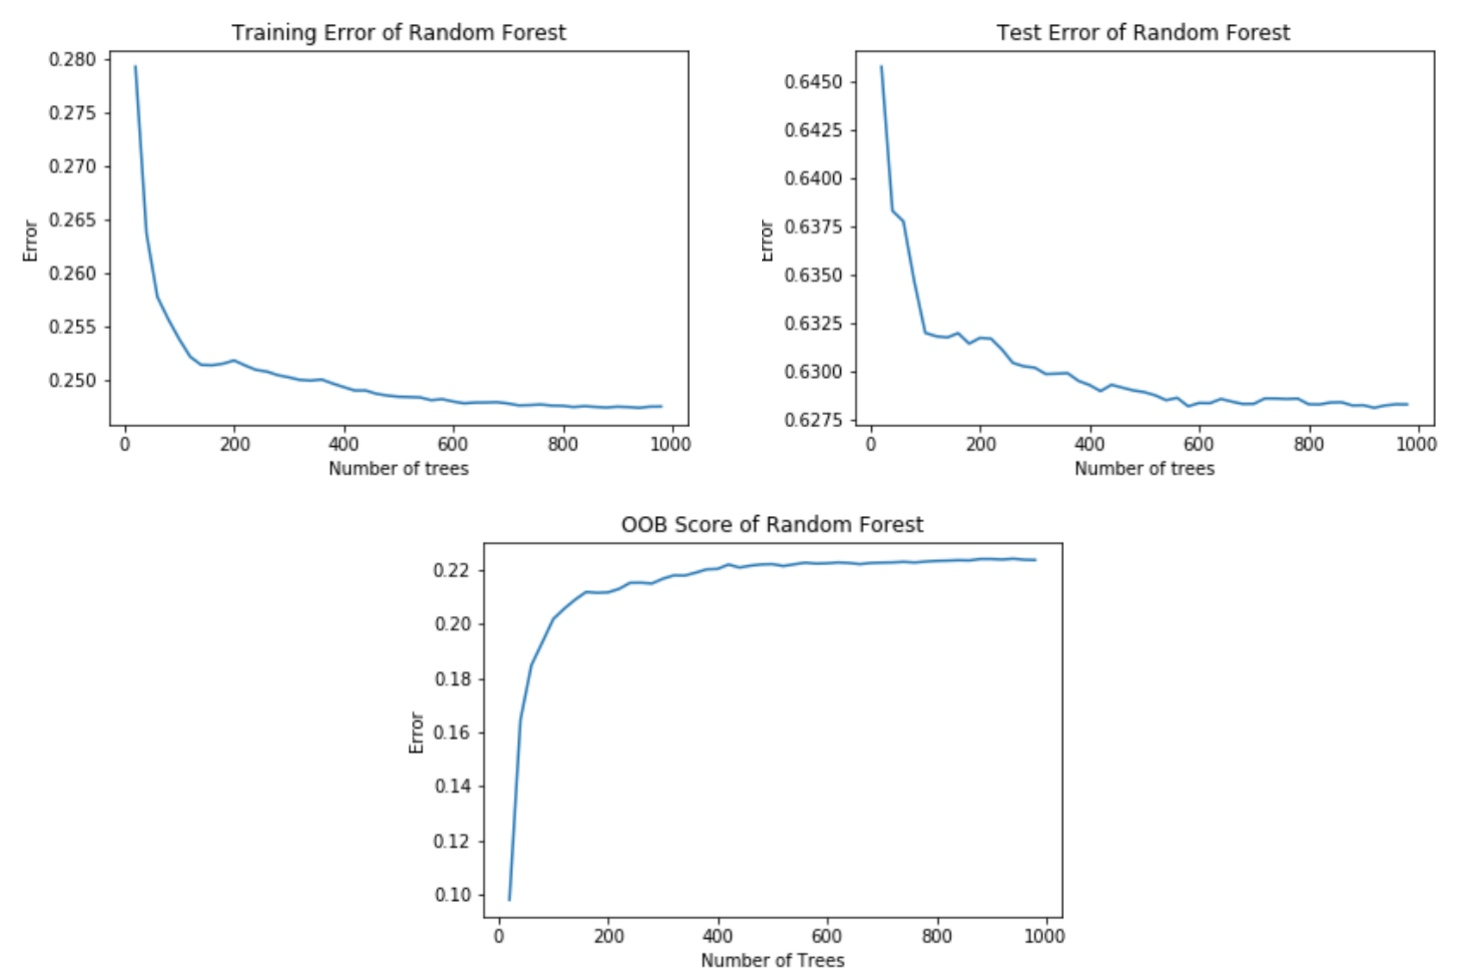
\includegraphics[width=9.5cm]{rf_error.jpg}}
\caption{Training Error, Test Error, and OOB score of the Random Forest}
\label{fig}
\end{figure}
\subsection{Neural Network}
The neural network used in this study is a multilayer perceptron based on scikit-learn MLPRegressor. We optimized this neural network by varying its hyperparameters and activation function to achieve minimum loss measured by RMSD. The optimal multilayer perceptron in this study has 90 neurons in its hidden layer with initial learning rate $l_r$ at 0.005, and the logistic sigmoid function as activation function.
\begin{figure}[htbp]
\centerline{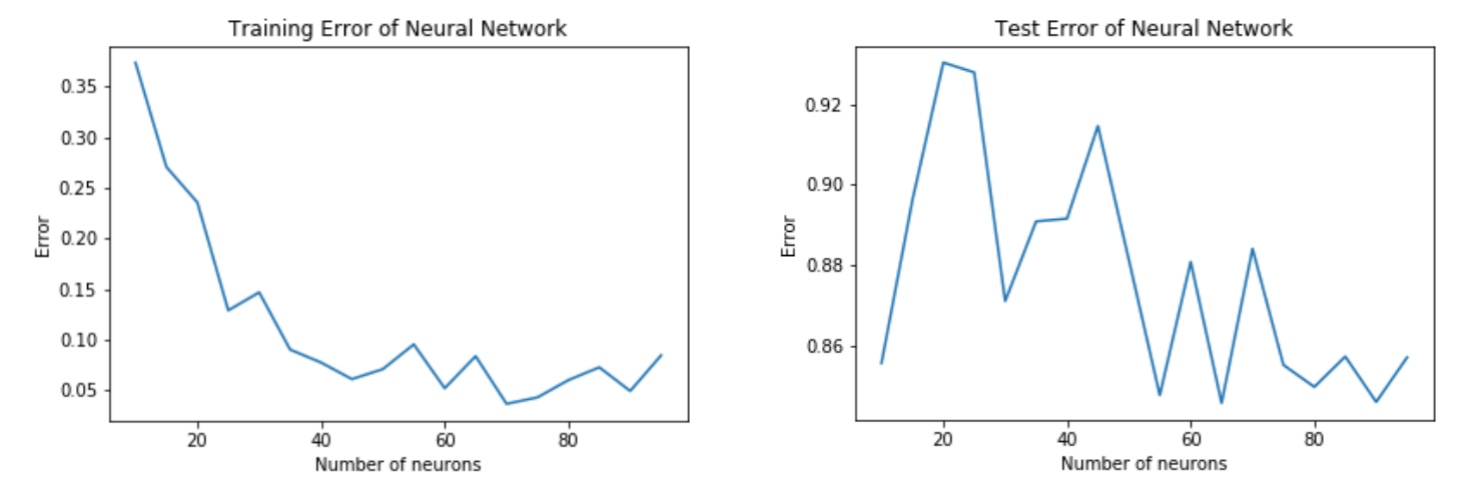
\includegraphics[width=9.5cm]{nn_error.jpg}}
\caption{Training Error and Test Error of the Neural Network}
\label{fig}
\end{figure}
\section{Experimental results and analysis}
In this section, top 10 principal factors that determine students' academic performance (measured by students’ standardized total exam scores) discovered respectively by linear regression, regression tree, and random forest are listed, explained, and compared in the first three subsections. Then, the fourth subsection uses the optimal multilayer perceptron neural network obtained during the experimental setup to evaluate the predictive performance of each set of principal factors. Finally, we change the target variable to students' cognitive test scores and standardized math, Chinese, and English exam scores to discuss whether principal factors affecting each subject are similar or different in the last subsection.
\subsection{Linear Regression}
The importance of each factor is scaled by the absolute value of its weight listed below in Table II. From Table II, principal factors that have the most positive effect on Chinese junior high school students' academic performance mainly lie in the \textit{Demographic} category, and parents apparently play a decisive role. Specifically, if a student's mother is ethnic minority or a member of the CCP, and his/her father has Bachelor degree, than he/she is more likely to be successful in his/her academic career. These factors are reasonable as China has preferential policies for minority students, and being a party member and having a Bachelor degree generally reflects a well-educated family background.

The importance of parents can also be consolidated by principal factors that have the most negative effect on students' academic performance. If they do not get along well, or if they do not care much about their child's experience (e.g. the student's relationship with his/her friends) in school, or if they have little confidence in their child, then they probably may undermine their child's learning motivation thus resulting in his/her poor academic performance. 

\begin{table}[htbp]
\caption{Top 10 Principal Factors Discovered by Linear Regression}
\begin{center}
\begin{tabular}{|c|c|c|c|}
\hline
\textbf{Variable}& \textbf{Meaning} & \textbf{Weight}\\
\hline
w2a05 & \makecell[l]{0-Student is not the only child of the family\\ 1-Student is the only child of the family} & \makecell[c]{-0.162356} \\
\hline
w2a17 & \makecell[l]{0-Parents get along very well \\1-Parents do not get along very well} & \makecell[c]{-0.120932}\\
\hline
w2a01 & \makecell[l]{0-Student's Hukou is in the local county \\1-Student's Hukou is not in the local county}  & \makecell[c]{-0.094967}\\
\hline
w2ba2602.1 & \makecell[l]{0-Parents often discuss the relationship \\ between his/her child and his/her friends \\1-Parents do not often discuss the \\ relationship between his/her child and \\ his/her friends } & \makecell[c]{-0.093424}\\
\hline
w2be11 & \makecell[l]{0-Mother is Han Chinese \\ 1-Mother is ethnic minority} & \makecell[c]{0.065215}\\
\hline
w2ba2602 & \makecell[l]{0-Parents often discuss with their child \\ things happened in school \\1-Parents do not often discuss with their \\child things happened in school } & \makecell[c]{-0.057533}\\
\hline
w2ba32.1 & \makecell[l]{0-Parents do not choose ``Not confident at \\all" with respect to their child's future \\1-Parents choose ``Not confident at all" with\\ respect to their child's future }  & \makecell[c]{-0.056092} \\
\hline
w2be16 & \makecell[l]{0-Mother is not a member of the CCP\\0-Mother is a member of the CCP}  & \makecell[c]{0.054267} \\
\hline
w2ba32.2 & \makecell[l]{0-Parents do not choose ``Not so confident"\\ with respect to their child's future \\1-Parents choose ``Not so confident" with \\respect to their child's future } & \makecell[c]{-0.050167} \\
\hline
w2be08 & \makecell[l]{0-Father does not have Bachelor degree \\ 1-Father has Bachelor degree}  & \makecell[c]{0.045347} \\
\hline
\end{tabular}
\label{tab1}
\end{center}
\end{table}
However, from Table II, the most crucial factor that negatively affects a student's academic performance is his/her one child status, which can be explained by the lack of peer companion. Besides, if a student's Hukou (household registration) status is not in the local county, then he/she may be allocated to an inferior school district, which will cast negative effect on his/her academic performance.

\subsection{Regression Tree}
Top 10 principal factors discovered by regression tree are summarized in Table III, where the importance of a specific feature is measured by the Gini importance, defined as the normalized loss reduction that feature brings [13]. 

Compared to Table II, they have a lot in common, but the major difference is that variables in Table III are all related to parents instead of students. The most significant factors are parents' educational background, requirement on their child's academic record, economic status, and ideal occupation of their child.  
\begin{table}[htbp]
\begin{center}
\caption{Top 10 Principal Factors Discovered by Regression Tree}
\begin{tabular}{|c|c|c|c|}
\hline
\textbf{Variable}& \textbf{Meaning} & \textbf{Importance}\\
\hline
w2ba29.2 & \makecell[l]{0-Parents do not expect Master/PhD \\degree as highest level of education \\1-Parents expects Master/PhD degree\\ as highest level of education} & \makecell[c]{0.452754} \\
\hline
w2a27 & \makecell[l]{0-Parents' requirement on their child's \\academic record is not ``Top five of the\\ class"\\ 1-Parents' requirement on their child's \\academic record is ``Top five of the class"} & \makecell[c]{0.183637}\\
\hline
w2a27.2 & \makecell[l]{0-Parents' requirement on their child's \\academic record is not ``About average"\\ 1-Parents' requirement on their child's \\academic record is ``About average"}  & \makecell[c]{0.141884}\\
\hline
w2be17 & \makecell[l]{0-Mother does not have Bachelor degree \\ 1-Mother has Bachelor degree} & \makecell[c]{0.120624}\\
\hline
w2ba30.3 & \makecell[l]{0-Parents do not most expect their \\child to become ``Government official, \\staff of public institutions, civil servant", \\``Manager or administrator of companies'',\\or ``Scientist/engineer/programmer/pilot''\\ in the future\\ 1-Parents most expects their child to\\ become ``Government official, staff of\\ public institutions, civil servant", \\``Manager or administrator of companies'',\\or ``Scientist/engineer/programmer/pilot''\\ in the future} & \makecell[c]{0.031678}\\
\hline
w2ba29.1 & \makecell[l]{0-Parents do not expect Bachelor degree\\ as highest level of education \\1-Parents expects Bachelor degree as\\ highest level of education} & \makecell[c]{0.025605}\\
\hline
w2be23.2 & \makecell[l]{0-Family's economic status is not at least\\ ``Moderate"\\ 1-Family's economic status is at least\\ ``Moderate"}  & \makecell[c]{0.019219} \\
\hline
w2be08 & \makecell[l]{0-Father does not have Bachelor degree \\ 1-Father has Bachelor degree}  & \makecell[c]{0.016788} \\
\hline
w2be11 & \makecell[l]{0-Mother is Han Chinese \\ 1-Mother is ethnic minority} & \makecell[c]{0.007810} \\
\hline
w2be07 & \makecell[l]{0-Father is not a member of the CCP\\0-Father is a member of the CCP} & \makecell[c]{0.007569} \\
\hline
\end{tabular}
\label{tab1}
\end{center}
\end{table}

Besides, Table III can also be visualized through Fig. 3—if a node is closer to the root node, then it has higher importance than other nodes.

\begin{figure}[htbp]
\centerline{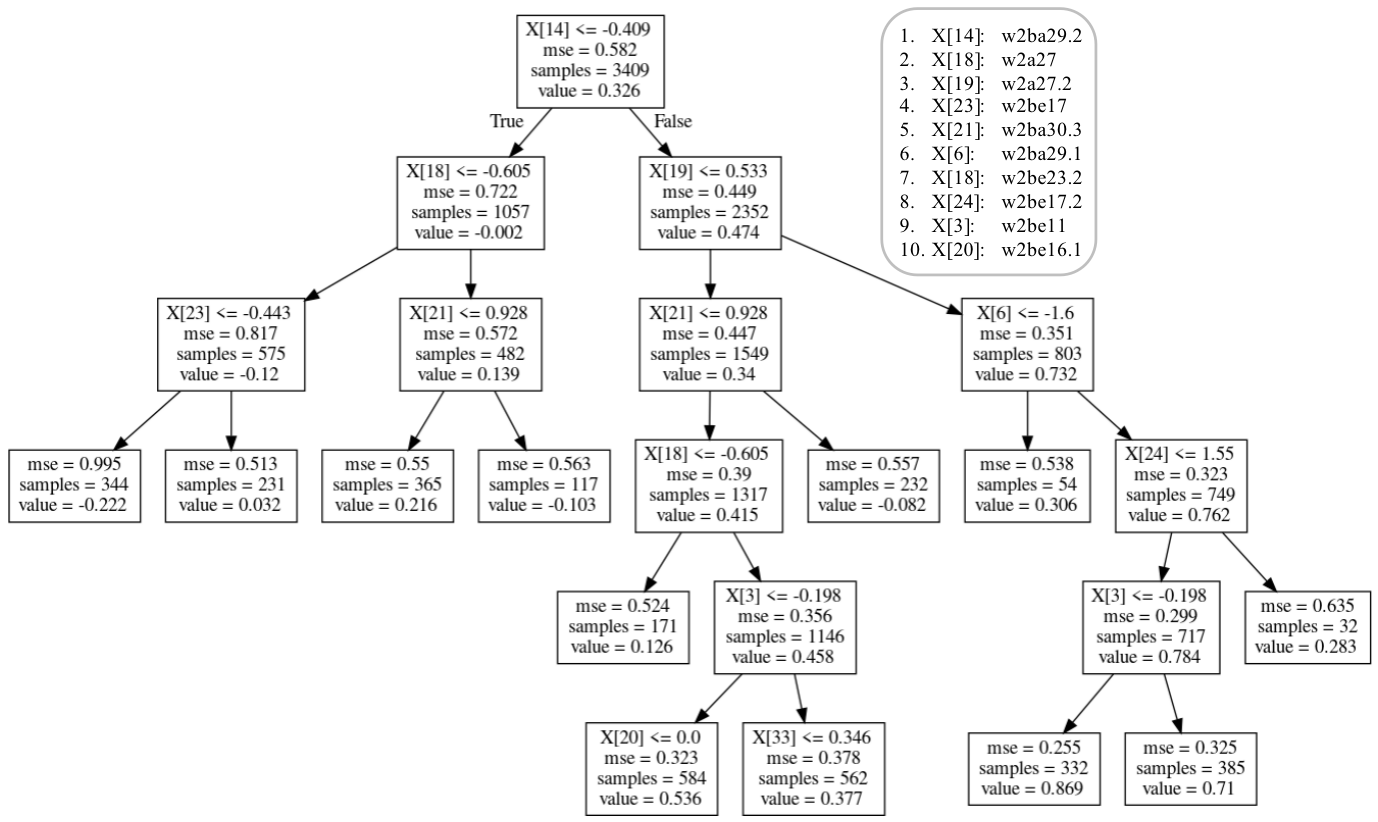
\includegraphics[width=9.40cm]{tree.png}}
\caption{Regression Tree}
\label{fig}
\end{figure}

\subsection{Random Forest}
Top 10 principal factors discovered by random forest are summarized in Table IV, where the importance of a specific feature is also measured by the Gini importance.
\begin{table}[htbp]
\begin{center}
\caption{Top 10 Principal Factors Discovered by Random Forest}
\begin{tabular}{|c|c|c|c|}
\hline
\textbf{Variable}& \textbf{Meaning} & \textbf{Importance}\\
\hline
w2b18.2 & \makecell[l]{0-Student does not expect Master/PhD\\degree as highest level of education\\1-Student expects Master/PhD degree as\\ highest level of education} & \makecell[c]{0.052732} \\
\hline
w2a27.2 & \makecell[l]{0-Parents' requirement on their child's\\academic record is not ``About average"\\ 1-Parents' requirement on their child's \\academic record is ``About average"} & \makecell[c]{0.040803}\\
\hline
w2a27 & \makecell[l]{0-Parents' requirement on their child's \\academic record is not ``Top 5 of the class"\\ 1-Parents' requirement on their child's \\academic record is ``Top 5 of the class"}  & \makecell[c]{0.040789}\\
\hline
w2ba29.2 & \makecell[l]{0-Parents do not expect Master/PhD degree\\as highest level of education \\1-Parents expects Master/PhD degree as\\ highest level of education} & \makecell[c]{0.021094}\\
\hline
w2a29.4 & \makecell[l]{0-Student does not feel ``Very stressed"\\ about parents' expectation \\1-Student feels ``Very stressed" about\\ parents' expectation} & \makecell[c]{0.011729}\\
\hline
w2bc0204 & \makecell[l]{0-Student did not receive government's \\subsidies last semester\\1-Student received government's subsidies\\ last semester} & \makecell[c]{0.011444}\\
\hline
w2a28.2 & \makecell[l]{0-Parents do not expect Master/PhD degree\\ as highest level of education\\1-Parents expect  Master/PhD degree as\\ highest level of education}  & \makecell[c]{0.011311} \\
\hline
w2a27.1 & \makecell[l]{0-Parents' requirement on their child's \\academic record is not ``Above average"\\ 1-Parents' requirement on their child's \\academic record is ``Above average"}  & \makecell[c]{0.009826} \\
\hline
w2be02 & \makecell[l]{0-Father is Han Chinese\\ 1-Father is ethnic minority} & \makecell[c]{0.007619} \\
\hline
w2be16 & \makecell[l]{0-Mother is not a member of the CCP\\0-Mother is a member of the CCP}  & \makecell[c]{0.007557} \\
\hline
\end{tabular}
\label{tab1}
\end{center}
\end{table}
\\

Compared to Table II and Table III, Table IV not only indicates parents' influence on their child, but also emphasizes the importance of a student's self-expectation—students with higher expectation for education and students under higher academic pressure have higher possibility to succeed.
\subsection{Comparison of Principal Factors with Respect to Different EDM Teniques}

After finishing the data mining process, we further evaluated the predictive performance of each set of principal factors by implementing the optimal multilayer perceptron neural network obtained from the experimental setup.
\begin{figure}[htbp]
\centerline{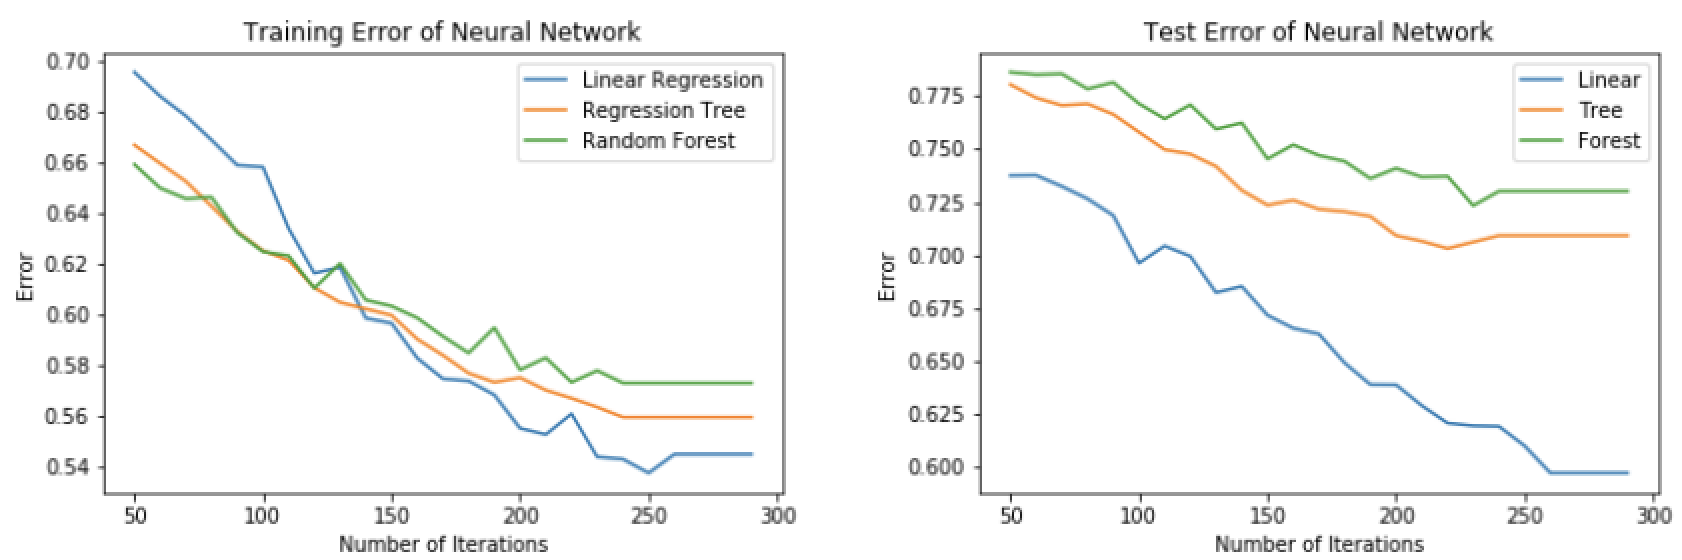
\includegraphics[width=9.5cm]{comparison.png}}
\caption{Predictive Performance Comparison of the Three Principal Factor Sets}
\label{fig}
\end{figure}

Fig. 4 demonstrates the principal factors selected by linear regression make training error and test error of the multilayer perceptron smallest, while the principal factors selected by random forest give the worst predictive performance. This result shows Table II summarizes the most accurate principal factors.

\subsection{Comparison of Principal Factors with Respect to Different Target Variables}
We changed the target variable from students' standardized total exam scores to their cognitive test scores and standardized math, Chinese, and English exam scores for further investigation. The results indicate that as for cognitive test scores, \textit{Willingness} accounts for the majority of principal factors; as for Chinese and English scores, the majority of principal factors are in the \textit{Interaction} category; while math score is largely influenced by the \textit{Demographic} variables. 

A logical explanation is that a student's cognitive ability is highly correlated to his/her academic test scores, such that the results obtained by setting cognitive test scores as the target variable are inclined to the results obtained by setting students' standardized total exam scores as the target variable. And because learning a language requires a lot of interaction and practice, so \textit{Interaction} has the most significant effect on Chinese and English scores. Finally, because of the difficulty of mathematics, it requires a lot of training and tutoring for students to learn math well. Therefore, for students from wealthier families, they have more opportunities to receive better mathematical education, and students' family background is clustered into the \textit{Demographic} category, so the data mining results show that math score is mainly determined by the \textit{Demographic} variables. 
\section{Conclusion}
In this study, we conducted Educational Data Mining (EDM) by linear regression, regression tree, random forest, and neural network on the China Education Panel Survey (CEPS) dataset. We clustered the CEPS dataset into three categories, namely, \textit{demographic and family background information (Demographic)}, \textit{self-perceived willingness for education (Willingness)}, and \textit{perceived family interaction (Interaction)}, and summarized principal factors that influence Chinese junoir high school students' academic performance. The linear regression model indicates that parents play a decisive role in their child's academic performance and reflects the significance of a student's Hukou status. The regression tree model further consolidates the importance of parents, while the random forest model shows that a student's self-expectation for education is also significant to his/her academic success. We evaluated the predictive performance of each set of principal factors by feeding these sets of principal factors into the optimal multilayer perceptron neural network we obtained during the experimental setup and comparing their training and test errors, and the result shows the principal factors selected by linear regression achieve the best predictive performance, while the principal factors selected by random forest give the worst predictive performance. Finally, we changed the target variable, and found that \textit{Willingness} largely accounts for students' cognitive test scores,  \textit{Demographic} mainly influences students' math scores, while \textit{Interaction} has the most significant effect on students' Chinese and English scores.

Based on our findings, we propose two practical strategies for China's educational inequality mitigation. First, students who have received government subsidies show higher potential to achieve better academic performance, so increase direct government subsidies to cover students' tuitions can create more equitable educational environment and encourage healthier competition. Second, decoupling school district from Hukou (household registration status) is also necessary since it allows non-local/immigrant students to share the same educational resources with local students. 

This study is the first comprehensive and quantitative investigation into the principal factors that affect Chinese junior high school students' academic performance on a national scale, but it is still recommendable for researchers to conduct more in-depth study in the future—more EDM techniques such as Hidden Markov Model (HMM) and collaborative filtering [6] could be applied, more datasets from different countries or regions could be taken into consideration, and more real-world educational surveys may be designed to substantiate the correctness of our findings.
\begin{thebibliography}{00}
\bibitem{b1} Sung Ho Ha, S. M. Bae, and S. C. Park. ``Web mining for distance education''. \textit{IEEE International Conference on Management of Innovation and Technology} IEEE, 2000.
\bibitem{b2} C. Romero and S. Ventura. ``Educational data mining: A survey from 1995 to 2005''. \textit{Expert Systems with Applications}, 33.1(2007): 135-146.
\bibitem{b3} Surjeet Kumar Yadav, B. Bharadwaj, and S. Pal. ``Data Mining Applications: A comparative Study for Predicting Student's Performance''. \textit{International Journal of Innovative Technology and Creative Engineering}, Vol.1 No.12 (2011): 13-19.
\bibitem{b4} Katrina Sin and L. Muthu. ``Application of big data in education data mining and learning analytics - a literature review''. \textit{ICTACT Journal on Soft Computing}, Vol 5. No.4 (2015): 1035-1049.
\bibitem{b5} Jiawei Han and M. Kamber. ``Data Mining: Concepts and Techniques'', \textit{The Morgan Kaufmann Series in Data Management Systems}, 2000.
\bibitem{b6} Alejandro Peña-Ayala. ``Electron spectroscopy studies on magneto-optical media and plastic substrate interface''. \textit{Expert Systems with Applications: An International Journal}, Vol.41 No.4 (2014): 1432–1462. 
\bibitem{b7} Q. A. Al-Radaideh, E. W. AI-Shawakfa, and M. I. AI-Najjar. ``Mining student data using decision trees''. \textit{International Arab Conference on Information Technology (ACIT)}, Yarmouk University, Jordan, 2006. 
\bibitem{b8} B. K. Bharadwaj and S. Pal. ``Data Mining: A prediction for performance improvement using classification''. \textit{International Journal of Computer Science and Information Security (IJCSIS)}, Vol.9 No.4 (2011): 136-140. 
\bibitem{b9} Lingxin Hao and Xiao Yu. ``Rural-Urban Migration and Children's Access to Education: China in Comparative Perspective''. Paper for \textit{The Education for All Global Monitoring Report}, 2015.
\bibitem{b10} Di Xu and Qiujie Li. ``Gender achievement gaps among Chinese middle school students and the role of teachers’ gender''. \textit{Economics of Education Review}, Vol.67 (2018): 82-93.
\bibitem{b11} Renming University of China. ``Academic Year 2014-2015 Student/Parent Questionnaire for Grade 8''. \textit{China Education Panel Survey (CEPS)}, 2015.
\bibitem{b12} T. Hastie, R. Tibshirani, and J. Friedman. ``The Elements of Statistical Learning (Second Edition, Corrected 12$^{th}$ Printing)''. \textit{Springer New York Inc.}, 2017.
\bibitem{b13} scikit-learn.org. ``sklearn.tree.DecisionTreeRegressor''. Web. $<$https://sc-\\ikit-learn.org/stable/modules/generated/sklearn.tree.DecisionTreeRegre-\\ss-or.html$>$. Accessed Jul. 30, 2017.
\end{thebibliography}
\end{document}